\documentclass[a4paper]{report}

% Preamble
\usepackage[spanish]{babel} % Paquete para utilizar el idioma español
\usepackage[utf8]{inputenc} % Codificación de caracteres UTF-8
\usepackage{setspace} % Para ajustar el espaciado entre líneas
\usepackage{titlesec} % Para personalizar los encabezados de capítulos y secciones
\usepackage{lipsum} % Para generar texto ficticio, puedes eliminar esta línea
\usepackage{enumitem} % Para enumerar items
\usepackage[hidelinks]{hyperref} % Para generar los enlaces a las secciones correspondientes
\usepackage{geometry}
\usepackage{graphicx}
\usepackage{fancyhdr}
\usepackage{microtype}
\usepackage{hyperref}
\usepackage{array}
\usepackage{chngcntr}
\usepackage{tocbibind}

% Otras configuraciones del preámbulo
\hypersetup{
  pdftitle={Sistema de Transmisión AM con Codificación DTMF},
  pdfauthor={Boeri, Benjamin; Campero, Leandro; Villafañe, Cristian},
  pdfsubject={Informe de Trabajo Integrador - Procesamiento Digital de Señales 2022},
  pdfkeywords={PDS, Informe, Boeri, Campero, Villafañe, 2022},
  pdfproducer={LaTeX},
  pdfcreator={pdfLaTeX}
}

% Header y footer
\pagestyle{fancy}
\fancyhf{}
\lhead{Procesamiento Digital de Señales}
\rhead{Trabajo Integrador}
\lfoot{\nouppercase{\leftmark}}
\rfoot{\thepage}

\fancypagestyle{plain}{
  \fancyhf{}
  \lhead{Procesamiento Digital de Señales}
  \rhead{Trabajo Integrador}
  \lfoot{\nouppercase{\leftmark}}
  \rfoot{\thepage}
}

\fancyhfoffset[R]{0pt} % Ajusta el ancho del encabezado
\fancyhfoffset[L]{0pt} % Ajusta el ancho del pie de página

\newgeometry{
  top=1.25in,
  bottom=1in,
  outer=0.75in,
  inner=0.75in,
}

% Configuración de página
\setlength{\parindent}{0pt} % Deshabilitar sangría al inicio de párrafos
\setlength{\parskip}{1em} % Establecer espaciado entre párrafos

% Personalizaciones
\titleformat{\chapter}[display]
{\normalfont\huge\bfseries}{\chaptertitlename\ \thechapter}{20pt}{\Huge}
\titlespacing*{\chapter}{0pt}{0pt}{40pt} % Ajustar espaciado antes y después de los encabezados de capítulo

% Tamaño de fuente e interlineado
\renewcommand{\normalsize}{\fontsize{12}{14}\selectfont}

\counterwithout{table}{section} % Desvincular el contador de las tablas de las secciones
\counterwithout{figure}{section} % Desvincular el contador de las figuras de las secciones
\counterwithin{table}{chapter} % Vincular el contador de las tablas al contador de los capítulos
\counterwithin{figure}{chapter} % Vincular el contador de las figuras al contador de los capítulos
\setlength{\tabcolsep}{10pt} % Espaciado horizontal
\setlength{\extrarowheight}{5pt} % Espaciado vertical

\newcommand{\titulo}{Sistema de Transmisión AM con Codificación DTMF}
\newcommand{\subtitulo}{Informe de Trabajo Integrador}
\newcommand{\materia}{Procesamiento Digital de Señales}
\newcommand{\unidadacademica}{Facultad de Ciencias Exactas y Tecnología}
\newcommand{\universidad}{Universidad Nacional de Tucumán}
\newcommand{\autores}{
  Boeri, Benjamin \\
  Campero, Leandro \\
  Villafañe, Cristian
}
\newcommand{\fecha}{\today}

% Comienza el documento
\begin{document}

% Página de título
\begin{titlepage}
  \centering


  \begin{spacing}{2}
    \textbf{\Huge \titulo}
  \end{spacing}

  \Large \subtitulo

  \vspace{1cm}

  
\includegraphics[width=6cm]{images/logo_unt.png}

  \textbf{\large \materia}

  \textbf{\large \unidadacademica}

  \textbf{\large \universidad}

  \vspace{0.5cm}

  \textbf{\Large Autores:}

  \autores

  \vfill

  \Large \fecha

\end{titlepage}

% Resumen
\begin{abstract}
  Aquí va el resumen.
\end{abstract}

% Índice
\tableofcontents

% Introduccion
% Capítulo 1
\chapter{Introducción}
\section{Problema propuesto}
La modulación en amplitud o \gls{am},
permite la transmisión de una señal de
baja frecuencia superpuesta a una onda
de alta frecuencia. Este sistema de
modulación permite enviar mensajes en
la forma de envolventes de la onda
portadora, ya sea por un canal de aire o
físico utilizando un enlace cableado.\\
El sistema de codificación \gls{dtfm}, utiliza una
combinación de tonos de frecuencia
audibles pera representar el conjunto de
números del 0 al 9 disponible en el
teclado telefónico, con lo cual es posible
enviar una codificación numérica por la
línea telefónica.\\
El modelo de trabajo está representado
en la Figura \ref{fig:intro_diagrama_bloques}, correspondientes al
Modulador y Demodulador \gls{am}, el canal
de cable telefónico, y las etapas de
codificación y decodificación \gls{dtfm}.

\begin{figure}[ht]
  \centering
  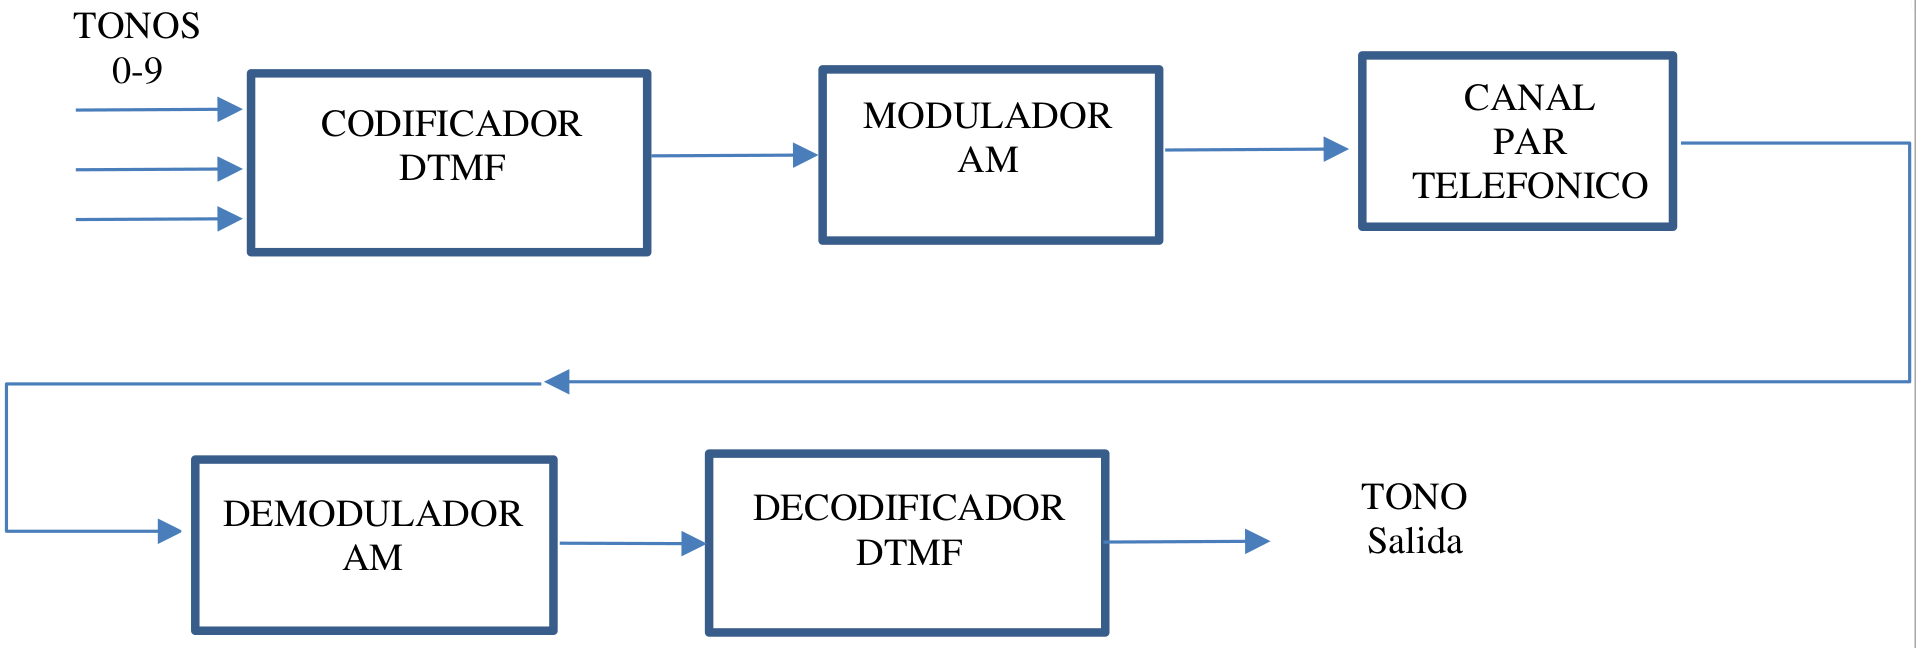
\includegraphics[width=\linewidth]{images/intro_diagrama_general.png}
  \caption{Diagrama de bloques general}
  \label{fig:intro_diagrama_bloques}
\end{figure}

\section{Objetivo}
El objetivo principal de este proyecto
integrador es la implementación del
sistema mostrado en la Figura \ref{fig:intro_diagrama_bloques},
utilizando MATLAB, SIMULINK, o la
combinación de ambos recursos de
modelado computacional, para el
envío de números (0-9) codificados
en \gls{dtfm} bajo modulación \gls{am}, y la
detección del número enviado a la
salida (uno número cada por vez).\\
A modo de referencia, el Cuadro \ref{tab:combinacion_tonos},
muestra la combinación de tonos
audibles asociados al conjunto
numérico, y en el enlace indicado
se encuentra la información ampliada
sobre la codificación \gls{dtfm}.

\begin{table}[htbp]
  \centering
  \begin{tabular}{|Sc|Sc|Sc|Sc|}
    \hline
    \textbf{Frecuencia Baja} & \textbf{Frecuencia Alta} & \textbf{Digito} & \textbf{Frecuencia Final} \\
    \hline
    697                      & 1209                     & 1               & 1906                      \\ \hline
    697                      & 1336                     & 2               & 2033                      \\ \hline
    697                      & 1477                     & 3               & 2174                      \\ \hline
    770                      & 1209                     & 4               & 1979                      \\ \hline
    770                      & 1336                     & 5               & 2106                      \\ \hline
    770                      & 1477                     & 6               & 2247                      \\ \hline
    852                      & 1209                     & 7               & 2061                      \\ \hline
    852                      & 1336                     & 8               & 2188                      \\ \hline
    852                      & 1477                     & 9               & 2329                      \\ \hline
    941                      & 1336                     & 0               & 2277                      \\
    \hline
  \end{tabular}
  \caption{Combinación de tonos audibles (medido en [Hz])}
  \label{tab:combinacion_tonos}
\end{table}

\section{Enunciado}
\begin{enumerate}[label=\alph*)]
  \item A nivel simulación se deberán sintetizar
        los tonos asociados a cada digito
        numérico seleccionando la frecuencia
        de muestreo $F_S$ apropiada (Teorema de Nyquist-Shannon).
  \item El demodulador \gls{dtfm} deberá ser
        implementado mediante filtros
        digitales pasa bandas, con un
        orden y respuestas apropiadas. El
        modo de indicar cuál fue el digito
        enviado queda a criterio del grupo
        de trabajo.
  \item Para el modelo de trasmisión AM
        (enlace cableado) se deberán
        establecer y sintetizar la frecuencia
        de portadora $RF$ el índice de
        modulación apropiados
        (recordando que la $F_S$ es única en
        todo el sistema).
  \item El canal de transmisión se
        corresponde al de un filtro
        analógico (transformado a digital)
        pasa banda con un rango de 300 Hz
        a 3400 Hz, respuesta plana y orden
        apropiado. Se considera el rango
        útil asignado a la frecuencia
        telefónica, aunque el cable
        telefónico de cobre tipo AWG-24,
        por ejemplo, supera este ancho de
        banda a 1Mz en distancias
        inferiores a 200 Mts.
\end{enumerate}

\section{Lineamientos Generales}
\begin{enumerate}[label=\alph*)]
  \item El grupo de trabajo deberá cumplir con las especificaciones del proyecto,
        utilizando criterios de diseños justificados para cada bloque del sistema.
  \item Se deberán indicar el paso a paso para el diseño de los filtros digitales utilizados
        en las diferentes etapas.
  \item El criterio de selección para el filtro analógico representativo del canal ( Bessel,
        Butterworth, etc.), y el método de transformación analógico a discreto escogido,
        brindando una gráfica comparativa de la respuesta en frecuencia resultantes en ambos
        planos (Laplace y Z).
  \item Se pide 3 aplicaciones posibles del sistema desarrollado en aplicaciones de tele
        comando (por ejemplo, aplicación de sistema de riego por comando telefónico de
        3 zonas), y como se imprentaría en la práctica (no el desarrollo, solo la propuesta).
  \item Problema de análisis: para el caso de que ocurran fallos en el canal de comunicación
        (por ejemplo, una atenuación en determinadas frecuencias), analizar la robustez del
        código detector para al menos 3 zonas atenuadas de frecuencias diferentes. Utilizar
        el código adjunto en Matlab para el diseño del canal con fallas. Justificar los
        resultados.
  \item Escribir el informe, Incluir conclusiones, observaciones y sugerencias sobre los
        resultados obtenidos
\end{enumerate}

\chapter{Revisión de literatura}
\section{Estudios anteriores}
Este capítulo contiene tu revisión de literatura.

\chapter{Metodología}
\section{Diseño de investigación}
Aquí explicas tu metodología de investigación.

% Añade más capítulos y secciones según sea necesario

% Conclusiones
\chapter{Conclusiones}
\section{Resumen de resultados}
Tu capítulo de conclusiones comienza aquí.

% Bibliografía
\begin{thebibliography}{}
  % Incluye tus referencias aquí
\end{thebibliography}

% Listado de figuras
\listoffigures

% Listado de tablas
\listoftables

% Apendices
\include{chapters/apendices}

\end{document}
